\documentclass[12pt, titlepage]{article}
\usepackage[utf8]{inputenc}
\usepackage{amsmath,amsthm,amsfonts,amssymb,amscd}
\usepackage{multirow,booktabs}
\usepackage[table]{xcolor}
\usepackage{fullpage}
\usepackage{lastpage}
\usepackage{enumitem}
\usepackage{fancyhdr}
\usepackage{mathrsfs}
\usepackage{wrapfig}
\usepackage{setspace}
\usepackage{calc}
\usepackage{multicol}
\usepackage{cancel}
\usepackage[retainorgcmds]{IEEEtrantools}
\usepackage[margin=3cm]{geometry}
\usepackage{amsmath}
\newlength{\tabcont}
\setlength{\parindent}{0.0in}
\setlength{\parskip}{0.05in}
\usepackage{empheq}
\usepackage{framed}
\usepackage[most]{tcolorbox}
\usepackage{xcolor}
\colorlet{shadecolor}{orange!15}
\parindent 0in
\parskip 12pt
\geometry{margin=1in, headsep=0.25in}
\theoremstyle{definition}
\newtheorem{defn}{Definition}
\newtheorem{reg}{Rule}
\newtheorem{exer}{Exercise}
\newtheorem{note}{Note}

\usepackage[american]{circuitikz}
\usepackage{bm}% Bold math
\usetikzlibrary{arrows.meta,decorations.markings}

\usepackage{mwe}
\usepackage{enumitem}
\usepackage[superscript,biblabel]{cite}
\usepackage{hyperref}
\hypersetup{colorlinks,linkcolor={blue},citecolor={blue},urlcolor={orange}}

\usepackage{graphicx}
% Path relative to the main .tex file
\graphicspath{ {./images/} }

\title{\textbf{Practical integrator using operational amplifier}}
\author{
  Russel Shawn Dsouza\\
  171EC143
  \and
  Sathvik S Prabhu\\
  171EC146
}
\date{13 November 2019}

% Vertical spacing for aligned equations
\setlength{\jot}{10pt}
% https://tex.stackexchange.com/a/42728
\newcommand\numberthis{\addtocounter{equation}{1}\tag{\theequation}}

\begin{document}
  \begin{titlepage}
    \begin{center}
      \LARGE{\textbf{Analog Integrated Circuits Lab}}\\
      \vspace*{2em}
      \LARGE{A Report on}\\
      \huge{\textbf{Practical integrator using operational amplifier}}\\
      \vspace*{1em}
      \LARGE{November 13, 2019}
    \end{center}

    \vspace*{2em}
    \hspace*{5em} \Large{Russel Shawn Dsouza} \hspace*{5em} \Large{Sathvik S. Prabhu}\\
    \hspace*{6em} \Large{171EC143} \hspace*{10em} \Large{171EC146}\\
    \vspace*{2em}
    \begin{center}
    
\includegraphics[scale=0.5]{logo.png}\\
    \vspace*{3em}
    Department of Electronics and Communication Engg.\\
    National Institute of Technology Karnataka, Surathkal\\
    Srinivasanagar 575 025, Karnataka, India
    \end{center}
  \end{titlepage}
  \thispagestyle{empty}

  \newpage
  \tableofcontents
  \thispagestyle{empty}

  \newpage
  \setcounter{page}{1}
  \section{Aim}
    To design, simulate, implement and test a $\mu$A741-based practical voltage integrator.

  \section*{Components required}
    \begin{itemize}
      \item $\mu$A741 op-amp
      \item Resistors R = 120k$\Omega$, 3.3k$\Omega$, 4.7k$\Omega$
      \item Capacitor C = 0.01 $\mu$F
      \item Signal generator
      \item Digital Storage Oscilloscope
      \item Breadboard
      \item Jumper wires
    \end{itemize}


  \newpage
  \section{Circuit diagram}
    \begin{figure}[h]
      \centering
      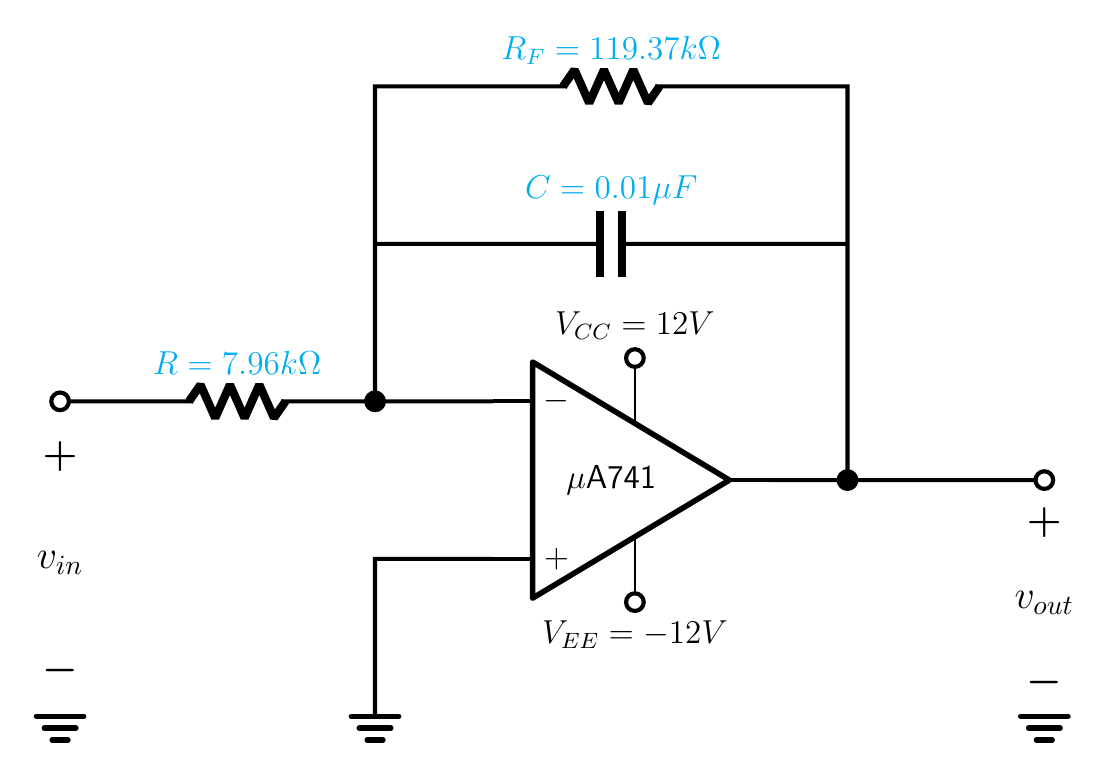
\begin{tikzpicture}[
        % Environment Config
        font=\large,
        MyArrow/.style={% Style for the current
          -Stealth,
          cyan,
          line width=1.5pt,
          shorten >= 5pt,
          shorten <= 1pt
        },
        Vref/.style={% Style for the voltage reference
          draw=none,
          postaction={decorate,decoration={markings,mark=at position 0.5 with {\node{\Large #1};}}},
          postaction={decorate,decoration={markings,mark=at position 0.15 with {\node{\Large $\bm{+}$};}}},
          postaction={decorate,decoration={markings,mark=at position 0.85 with {\node{\Large $\bm{-}$};}}}
        },
        Numbered/.style = {% Style for circle marks
          draw,
          circle,
          line width=1.5pt,
          align=center,
          inner sep=4pt,
          label distance=15pt
        }
      ]

      \def\MyOpamp(#1)#2{% Custom opamp
        \begin{scope}[shift={(#1)}]
          %===Component Shape===
          \draw[line width = 2pt, line join=round] (0,0)++(-1,1.5)
            --++(2.5,-1.5) -- ++(-2.5,-1.5)-- cycle;
          %===Label===
          \draw(0,0) node{\sf $\mu$A741};
          %===PIN: IN-===
          \draw[line width = 1.5pt] (-1,1) node [anchor=180]{$-$} -- ++(-0.5,0)  coordinate (#2 IN-);
          %===PIN: N+===
          \draw[line width = 1.5pt] (-1,-1) node [anchor=180]{$+$}  -- ++(-0.5,0) coordinate (#2 IN+);
          %===PIN: OUT===
          \draw[line width = 1.5pt] (1.5,0)  -- ++(0.5,0) coordinate (#2 OUT);
          %===PIN: Vcc===
          \draw[line width = 1pt] (0.3, 0.75) -- ++(0, 0.8) coordinate (#2 Vcc);
          \draw(0.3,1.55) node[ocirc,scale=2,line width=1.5pt, label=above:${V_{CC} = 12V}$]{};
          %===PIN: Vee===
          \draw[line width = 1pt] (0.3, -0.75) -- ++(0, -0.8) coordinate (#2 Vee);
          \draw(0.3,-1.55) node[ocirc,scale=2,line width=1.5pt, label=below:${V_{EE} = -12V}$]{};
        \end{scope}
      }
      \def\MyGround(#1)#2{% Customized Ground
        \begin{scope}[shift={(#1)}]
          % Component Shape
          \draw[line width = 2pt, line cap=round]
          (0,0) coordinate (#2 GND)++(-0.3,0)--++(0.6,0)
          (0,-0.15)++(-0.2,0)--++(0.4,0)
          (0,-0.3)++(-0.1,0)--++(0.2,0);
        \end{scope}
      }

      % Put the customzed opamp in position
      \MyOpamp(0,0){1}

      % Put some short nodes
      \draw(-7,1) node[ocirc,scale=2,line width=1.5pt](N3){};
      \draw(-3,1) node[circ,scale=2,line width=1.5pt](N2){};
      \draw(3,0) node[circ,scale=2,line width=1.5pt](N6){};
      \draw(5.5,0) node[ocirc,scale=2,line width=1.5pt](N6-OUT){};
      \MyGround(-7,-3){1}
      \MyGround(1 GND -| N2){2}
      \MyGround(1 GND -| N6-OUT){3}

      % Draw the Wires and pasive components
      \draw[line width=1.5pt]
      (N3)%From node N3
          --++(0.5,0)
          to [R,l=\color{cyan}\large${R = 7.96k\Omega}$] (N2)
          --(1 IN-)
      (N2)
          --++(0,2) coordinate (N5)
          --++(1.5,0)
          to[C,l=\color{cyan}\large${C = 0.01\mu F}$]++(3,0)
          -| (N6)
      (N2)
          --++(0, 4) coordinate (NRf)
          --++(1.5, 0)
          to[R,l=\color{cyan}\large${R_F = 119.37k\Omega}$]++(3,0)
          -| (N6)
      (1 OUT)
          -- (N6-OUT)
      (1 IN+)
          -|(2 GND);

      % Voltage references
      %===Vin===
      \draw[Vref=$v_{in}$]
      (N3)
          -- (1 GND);

      % %===Vd===
      % \draw[Vref=$V_d$,color=cyan]
      % (1 IN-)
      %     ++(-0.5,0) coordinate (temp)
      %     -- (1 IN+ -| temp)
      %     node[
      %         midway,
      %     ]{};

      %===Vout===
      \draw[Vref=$v_{out}$]
      (N6-OUT)
          -- (3 GND);
          % ===Equation:Vout===
          % node [
          %     midway,
          %     % label={[Numbered,black,label distance=5pt]180:\bf 6}
          % ]{$\bm{v_{out}}$};

      % %===Virtual Ground===
      % \draw[MyArrow]
      % (N2)++(-1.5,-5)
      %     node [](C1){$\bm{v_p} = \bm{v_n} = 0$ \bf (Virtual ground)}
      % (C1.168) %get a point from center to node box at 168 degrees
      %     to [out=80, in=-150] (N2);

      % Draw currents
      % %===Iin===
      % \draw[MyArrow]
      % (N3)++(0.3,0.3)
      %     -- ++(1.5,0)
      %     node [
      %         midway,
      %         inner sep=10pt,
      %         anchor=-70,
      %         % label={[Numbered,black,label distance=0pt]180:\bf 3}
      %     ]{$\bm{i_{in}} = \cfrac{\bm{v_{in}}}{R}$};

      % %===Ic===
      % \draw[MyArrow]
      % (N5)++(0.3,0.3) %node gap
      %     -- ++(2,0) % Arrow longitude
      %     node [
      %         midway,
      %         inner sep=10pt,
      %         anchor=-80,
      %         % label={[Numbered,black,label distance=0pt]180:\bf 5}
      %     ]{$\bm{i_C}$};

      % %===Irf===
      % \draw[MyArrow]
      % (NRf)++(0.3,0.3) %node gap
      %     -- ++(2,0) % Arrow longitude
      %     node [
      %         midway,
      %         inner sep=10pt,
      %         anchor=-80,
      %         % label={[Numbered,black,label distance=0pt]180:\bf 5}
      %     ]{$\bm{i_{R_F}}$};

      \end{tikzpicture}
      \caption{Circuit showing the final design}
      \label{fig:designed_practical_integrator}
    \end{figure}

    % Uncomment to include LTSpice circuit
    % \begin{figure}[h]
    %   \centering
    %   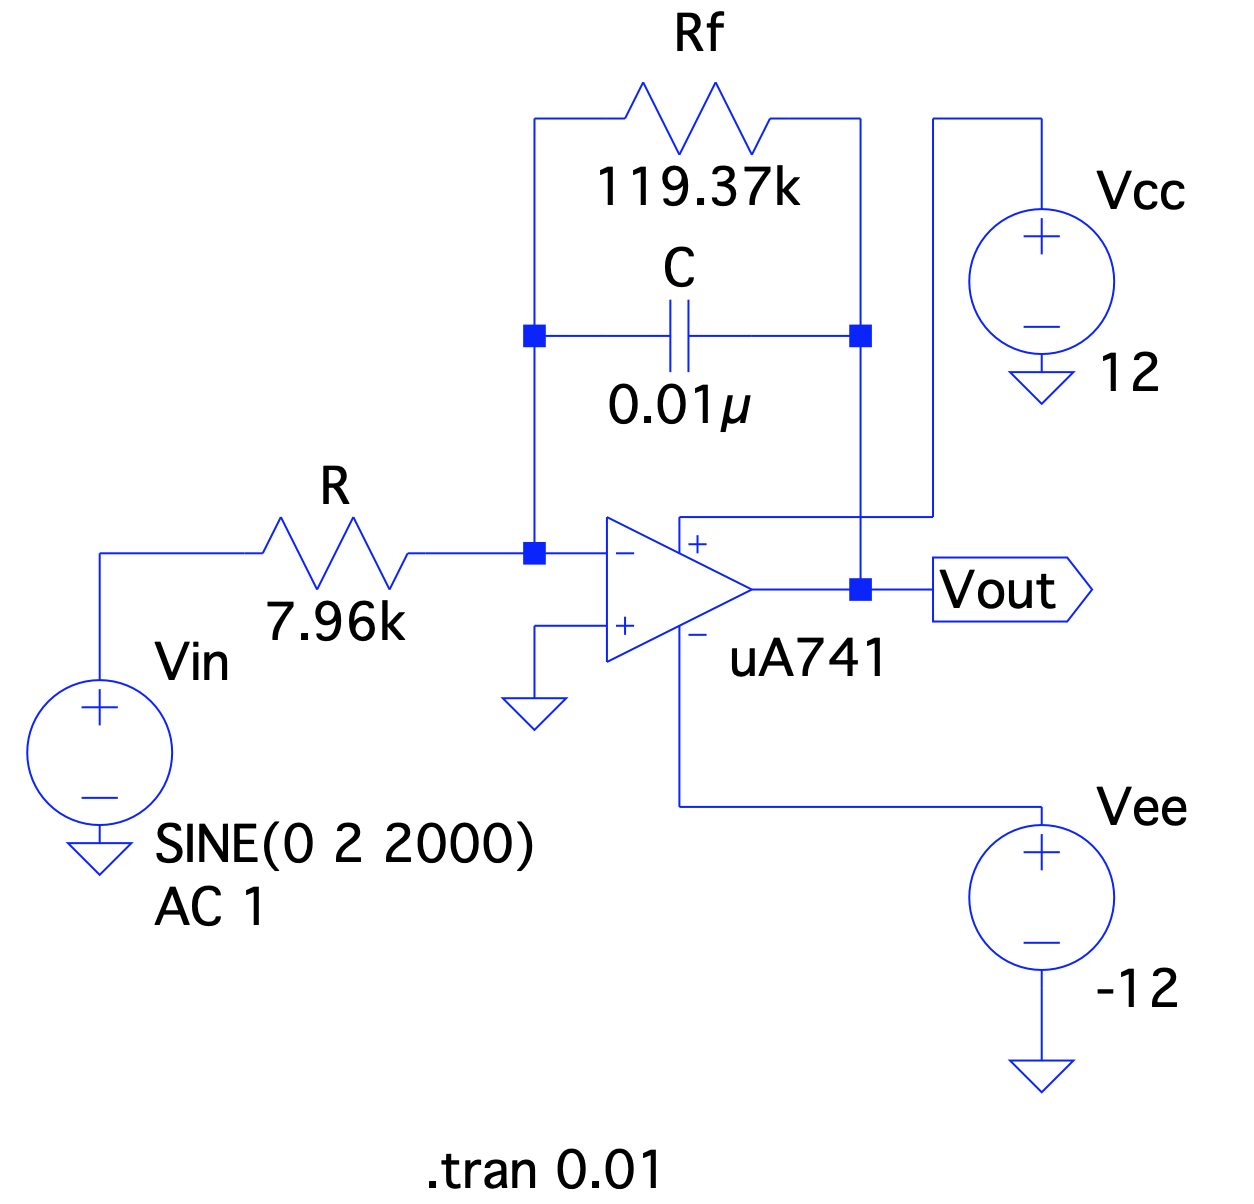
\includegraphics[scale=0.3]{images/sim_circuit.png}
    %   \caption{Circuit as drafted on LTSpice}
    % \end{figure}

  \newpage
  \section{Theory}
    %===Basics of op-amp integrator===
    The operational amplifier based integrator performs the mathematical operation of integration with respect to time, i.e. its output is proportional to the input voltage integrated over time.
    The integrator circuit is mostly used in analog computers, analog-to-digital converters and wave-shaping circuits such as charge amplifiers.

    The response of an op-amp circuit with feedback reflects the characteristics of the feedback elements. Thus, in order to achieve integration, the feedback network is constructed using a capacitor.

    %===Ideal op-amp integrator===
    An operational amplifier based integrator can ideally be constructed as shown in figure \ref{fig:theoretical_ideal_integrator}.

      \begin{figure}[h]
        \centering
        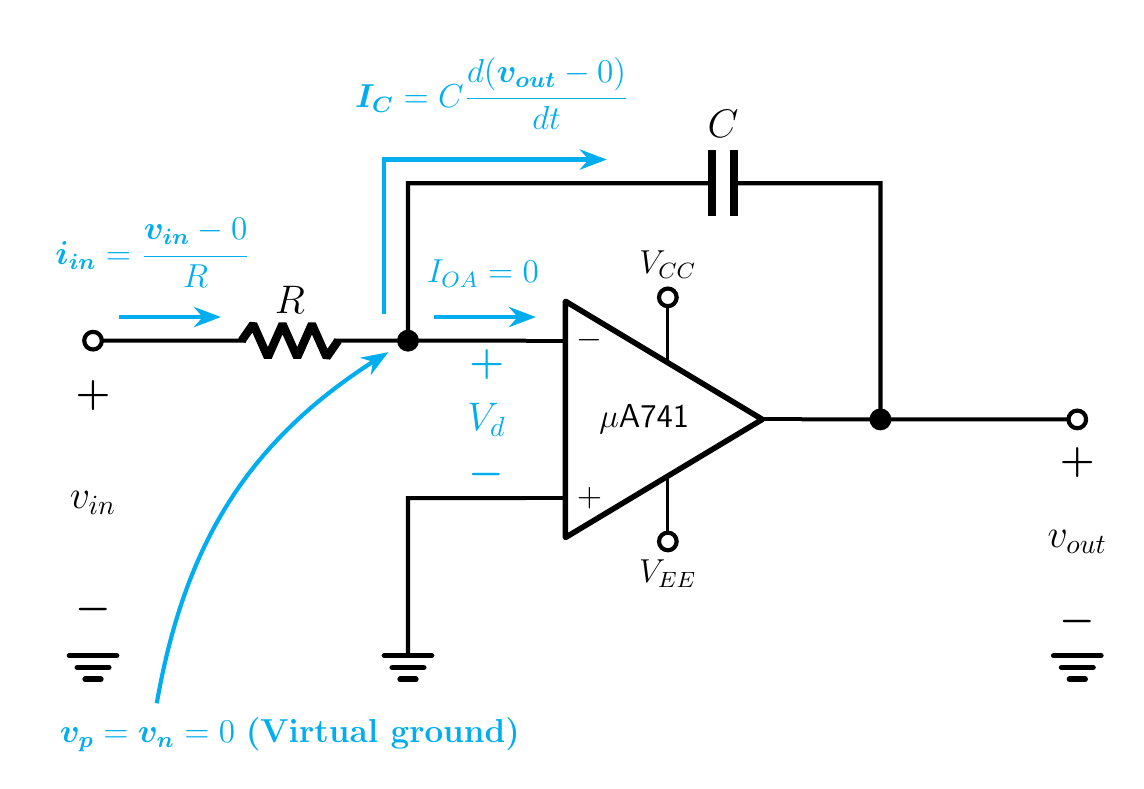
\begin{tikzpicture}[
          % Environment Config
          font=\large,
          MyArrow/.style={% Style for the current
            -Stealth,
            cyan,
            line width=1.5pt,
            shorten >= 5pt,
            shorten <= 1pt
          },
          Vref/.style={% Style for the voltage reference
            draw=none,
            postaction={decorate,decoration={markings,mark=at position 0.5 with {\node{\Large #1};}}},
            postaction={decorate,decoration={markings,mark=at position 0.15 with {\node{\Large $\bm{+}$};}}},
            postaction={decorate,decoration={markings,mark=at position 0.85 with {\node{\Large $\bm{-}$};}}}
          },
          Numbered/.style = {% Style for circle marks
            draw,
            circle,
            line width=1.5pt,
            align=center,
            inner sep=4pt,
            label distance=15pt
          }
        ]

        \def\MyOpamp(#1)#2{% Custom opamp
          \begin{scope}[shift={(#1)}]
            %===Component Shape===
            \draw[line width = 2pt, line join=round] (0,0)++(-1,1.5)
              --++(2.5,-1.5) -- ++(-2.5,-1.5)-- cycle;
            %===Label===
            \draw(0,0) node{\sf $\mu$A741};
            %===PIN: IN-===
            \draw[line width = 1.5pt] (-1,1) node [anchor=180]{$-$} -- ++(-0.5,0)  coordinate (#2 IN-);
            %===PIN: N+===
            \draw[line width = 1.5pt] (-1,-1) node [anchor=180]{$+$}  -- ++(-0.5,0) coordinate (#2 IN+);
            %===PIN: OUT===
            \draw[line width = 1.5pt] (1.5,0)  -- ++(0.5,0) coordinate (#2 OUT);
            %===PIN: Vcc===
            \draw[line width = 1pt] (0.3, 0.75) -- ++(0, 0.8) coordinate (#2 Vcc);
            \draw(0.3,1.55) node[ocirc,scale=2,line width=1.5pt, label=above:$V_{CC}$]{};
            %===PIN: Vee===
            \draw[line width = 1pt] (0.3, -0.75) -- ++(0, -0.8) coordinate (#2 Vee);
            \draw(0.3,-1.55) node[ocirc,scale=2,line width=1.5pt, label=below:$V_{EE}$]{};
          \end{scope}
        }
        \def\MyGround(#1)#2{% Customized Ground
          \begin{scope}[shift={(#1)}]
            % Component Shape
            \draw[line width = 2pt, line cap=round]
            (0,0) coordinate (#2 GND)++(-0.3,0)--++(0.6,0)
            (0,-0.15)++(-0.2,0)--++(0.4,0)
            (0,-0.3)++(-0.1,0)--++(0.2,0);
          \end{scope}
        }

        % Put the customzed opamp in position
        \MyOpamp(0,0){1}

        % Put some short nodes
        \draw(-7,1) node[ocirc,scale=2,line width=1.5pt](N3){};
        \draw(-3,1) node[circ,scale=2,line width=1.5pt](N2){};
        \draw(3,0) node[circ,scale=2,line width=1.5pt](N6){};
        \draw(5.5,0) node[ocirc,scale=2,line width=1.5pt](N6-OUT){};
        \MyGround(-7,-3){1}
        \MyGround(1 GND -| N2){2}
        \MyGround(1 GND -| N6-OUT){3}

        % Draw the Wires and pasive components
        \draw[line width=1.5pt]
        (N3)%From node N3
            --++(1,0)
            to [R,l=\Large$R$] (N2)
            --(1 IN-)
        (N2)
            --++(0,2) coordinate (N5)
            --++(2.5,0)
            to[C,l=\Large$C$]++(3,0)
            -| (N6)
        (1 OUT)
            -- (N6-OUT)
        (1 IN+)
            -|(2 GND);

        % Voltage references
        %===Vin===
        \draw[Vref=$v_{in}$]
        (N3)
            -- (1 GND);

        %===Vd===
        \draw[Vref=$V_d$,color=cyan]
        (1 IN-)
            ++(-0.5,0) coordinate (temp)
            -- (1 IN+ -| temp)
            node[
                midway,
            ]{};

        %===Vout===
        \draw[Vref=$v_{out}$]
        (N6-OUT)
            -- (3 GND);

        %===Virtual Ground===
        \draw[MyArrow]
        (N2)++(-1.5,-5)
            node [](C1){$\bm{v_p} = \bm{v_n} = 0$ \bf (Virtual ground)}
        (C1.168) %get a point from center to node box at 168 degrees
            to [out=80, in=-150] (N2);

        % Draw currents
        %===Iin===
        \draw[MyArrow]
        (N3)++(0.3,0.3)
            -- ++(1.5,0)
            node [
                midway,
                inner sep=10pt,
                anchor=-70,
                % label={[Numbered,black,label distance=0pt]180:\bf 3}
            ]{$\bm{i_{in}} = \cfrac{\bm{v_{in}} - 0}{R}$};

        %===Ic===
        \draw[MyArrow]
        (N2)++(-0.3, 0.3) %node gap
            -- ++(0, 2)
            -- ++(3, 0) % Arrow longitude
            node [
              midway,
              inner sep = 10pt,
              anchor = -80,
            ]{$\bm{I_C} = C\cfrac{d(\bm{v_{out}} - 0)}{dt}$};

        %===Ioa===
        \draw[MyArrow]
        (N2)++(0.3, 0.3)
            -- ++(1.5, 0)
            node [
              midway,
              inner sep = 10pt,
              anchor = -80
            ]{$I_{OA} = 0$};

        \end{tikzpicture}
        \caption{Ideal opamp integrator}
        \label{fig:theoretical_ideal_integrator}
      \end{figure}

    The circuit can be analysed by applying Kirchhoff's current law at the node $V_n$, keeping ideal op-amp behaviour in mind.
    \begin{equation}\label{eq:ideal_kcl_vn}
      i_{in} = I_C = \cfrac{V_{in}}{R}
    \end{equation}

    The relationship between between the capacitor's voltage and current is modelled as:
    \begin{equation}\label{eq:ideal_i-v_cap}
      I_C = C\cfrac{dV_C}{dt}
    \end{equation}

    Substituting eq. \ref{eq:ideal_kcl_vn} in eq. \ref{eq:ideal_i-v_cap}:
    \begin{align*}
      \cfrac{v_{in} - 0}{R} &= C\cfrac{d(0 - v_{out})}{dt}
      \implies \cfrac{v_{in}}{R} = -C\cfrac{dv_{out}}{dt}
    \end{align*}

    Integrating both sides with respect to time:
    \begin{align*}
      \int_0^t {\cfrac{v_{in}}{R}} &= - \int_0^t {\cfrac{dv_{out}}{dt}dt} \\
      v_{out} &= -\cfrac{1}{RC} \int_0^t {v_{in}{dt}}
    \end{align*}
    Thus the output of the circuit shown in figure \ref{fig:theoretical_ideal_integrator} is the inverted, integrated input with a gain of $\cfrac{1}{RC}$.

    %===Limitations of ideal integrator===
    The ideal integrator suffers from two main limitations. One comes from the fact that the output volatage of the op-amp cannot exceed the supply voltage.
    The output of the integrator is inversely proportional to the time constant $\tau = RC$.
    The larger the time constant $\tau$ ,the longer it takes to saturate the integrator.
    The second limitation is a consequence of the offset voltage present even for zero input.
    It may be only a few milivolts, but this gets integrated over time and it eventually drives the op-amp to saturation.

    %===Practical op-amp integrator===
    One can overcome the limitations of an ideal integrator by adding a resistor $R_{f}$ in parallel with capacitor $C$ as shown in figure \ref{fig:theoretical_practical_integrator}. $R_{f}$ prevents the op-amp from going into open loop configuration at low frequencies.

    \begin{figure}[h]
      \centering
      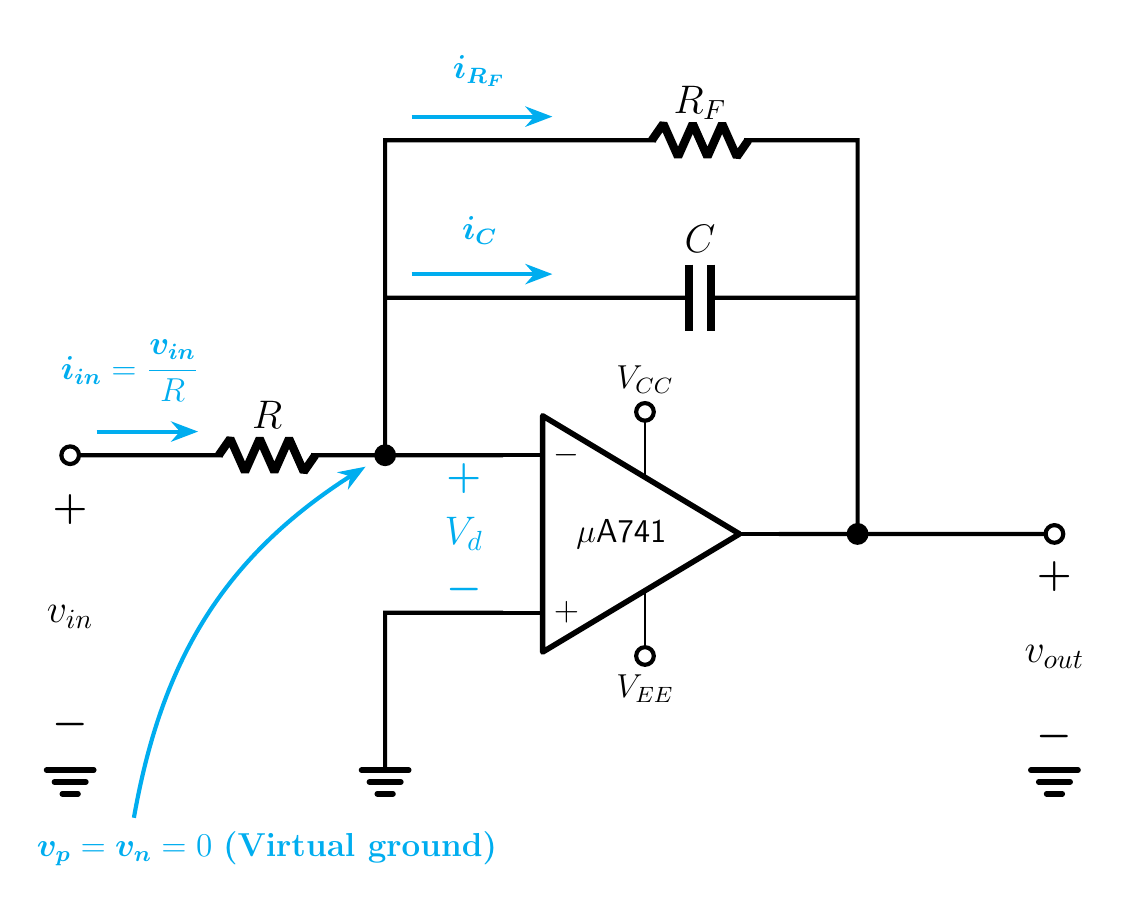
\begin{tikzpicture}[
        % Environment Config
        font=\large,
        MyArrow/.style={% Style for the current
          -Stealth,
          cyan,
          line width=1.5pt,
          shorten >= 5pt,
          shorten <= 1pt
        },
        Vref/.style={% Style for the voltage reference
          draw=none,
          postaction={decorate,decoration={markings,mark=at position 0.5 with {\node{\Large #1};}}},
          postaction={decorate,decoration={markings,mark=at position 0.15 with {\node{\Large $\bm{+}$};}}},
          postaction={decorate,decoration={markings,mark=at position 0.85 with {\node{\Large $\bm{-}$};}}}
        },
        Numbered/.style = {% Style for circle marks
          draw,
          circle,
          line width=1.5pt,
          align=center,
          inner sep=4pt,
          label distance=15pt
        }
      ]

      \def\MyOpamp(#1)#2{% Custom opamp
        \begin{scope}[shift={(#1)}]
          %===Component Shape===
          \draw[line width = 2pt, line join=round] (0,0)++(-1,1.5)
            --++(2.5,-1.5) -- ++(-2.5,-1.5)-- cycle;
          %===Label===
          \draw(0,0) node{\sf $\mu$A741};
          %===PIN: IN-===
          \draw[line width = 1.5pt] (-1,1) node [anchor=180]{$-$} -- ++(-0.5,0)  coordinate (#2 IN-);
          %===PIN: N+===
          \draw[line width = 1.5pt] (-1,-1) node [anchor=180]{$+$}  -- ++(-0.5,0) coordinate (#2 IN+);
          %===PIN: OUT===
          \draw[line width = 1.5pt] (1.5,0)  -- ++(0.5,0) coordinate (#2 OUT);
          %===PIN: Vcc===
          \draw[line width = 1pt] (0.3, 0.75) -- ++(0, 0.8) coordinate (#2 Vcc);
          \draw(0.3,1.55) node[ocirc,scale=2,line width=1.5pt, label=above:$V_{CC}$]{};
          %===PIN: Vee===
          \draw[line width = 1pt] (0.3, -0.75) -- ++(0, -0.8) coordinate (#2 Vee);
          \draw(0.3,-1.55) node[ocirc,scale=2,line width=1.5pt, label=below:$V_{EE}$]{};
        \end{scope}
      }
      \def\MyGround(#1)#2{% Customized Ground
        \begin{scope}[shift={(#1)}]
          % Component Shape
          \draw[line width = 2pt, line cap=round]
          (0,0) coordinate (#2 GND)++(-0.3,0)--++(0.6,0)
          (0,-0.15)++(-0.2,0)--++(0.4,0)
          (0,-0.3)++(-0.1,0)--++(0.2,0);
        \end{scope}
      }

      % Put the customzed opamp in position
      \MyOpamp(0,0){1}

      % Put some short nodes
      \draw(-7,1) node[ocirc,scale=2,line width=1.5pt](N3){};
      \draw(-3,1) node[circ,scale=2,line width=1.5pt](N2){};
      \draw(3,0) node[circ,scale=2,line width=1.5pt](N6){};
      \draw(5.5,0) node[ocirc,scale=2,line width=1.5pt](N6-OUT){};
      \MyGround(-7,-3){1}
      \MyGround(1 GND -| N2){2}
      \MyGround(1 GND -| N6-OUT){3}

      % Draw the Wires and pasive components
      \draw[line width=1.5pt]
      (N3)%From node N3
          --++(1,0)
          to [R,l=\Large$R$] (N2)
          --(1 IN-)
      (N2)
          --++(0,2) coordinate (N5)
          --++(2.5,0)
          to[C,l=\Large$C$]++(3,0)
          -| (N6)
      (N2)
          --++(0, 4) coordinate (NRf)
          --++(2.5, 0)
          to[R,l=\Large$R_F$]++(3,0)
          -| (N6)
      (1 OUT)
          -- (N6-OUT)
      (1 IN+)
          -|(2 GND);

      % Voltage references
      %===Vin===
      \draw[Vref=$v_{in}$]
      (N3)
          -- (1 GND);

      %===Vd===
      \draw[Vref=$V_d$,color=cyan]
      (1 IN-)
          ++(-0.5,0) coordinate (temp)
          -- (1 IN+ -| temp)
          node[
              midway,
          ]{};

      %===Vout===
      \draw[Vref=$v_{out}$]
      (N6-OUT)
          -- (3 GND);
          % ===Equation:Vout===
          % node [
          %     midway,
          %     % label={[Numbered,black,label distance=5pt]180:\bf 6}
          % ]{$\bm{v_{out}}$};

      %===Virtual Ground===
      \draw[MyArrow]
      (N2)++(-1.5,-5)
          node [](C1){$\bm{v_p} = \bm{v_n} = 0$ \bf (Virtual ground)}
      (C1.168) %get a point from center to node box at 168 degrees
          to [out=80, in=-150] (N2);

      % Draw currents
      %===Iin===
      \draw[MyArrow]
      (N3)++(0.3,0.3)
          -- ++(1.5,0)
          node [
              midway,
              inner sep=10pt,
              anchor=-70,
              % label={[Numbered,black,label distance=0pt]180:\bf 3}
          ]{$\bm{i_{in}} = \cfrac{\bm{v_{in}}}{R}$};

      %===Ic===
      \draw[MyArrow]
      (N5)++(0.3,0.3) %node gap
          -- ++(2,0) % Arrow longitude
          node [
              midway,
              inner sep=10pt,
              anchor=-80,
              % label={[Numbered,black,label distance=0pt]180:\bf 5}
          ]{$\bm{i_C}$};

      %===Irf===
      \draw[MyArrow]
      (NRf)++(0.3,0.3) %node gap
          -- ++(2,0) % Arrow longitude
          node [
              midway,
              inner sep=10pt,
              anchor=-80,
              % label={[Numbered,black,label distance=0pt]180:\bf 5}
          ]{$\bm{i_{R_F}}$};

      \end{tikzpicture}
      \caption{Practical op-amp integrator}
      \label{fig:theoretical_practical_integrator}
    \end{figure}

    The resulting circuit is an inverting amplifier with $R_F||\cfrac{1}{Cs}$ acting as the feedback resistance.
    The gain of such an amplifier is given by:
    \begin{align*}
      \cfrac{V_{out}(s)}{V_{in}(s)} &= - \cfrac{R_F||\cfrac{1}{Cs}}{R}\\
      &= - \cfrac{R_F}{R} \cfrac{1}{(1 + R_F Cs)}
    \end{align*}

    Thus, the frequency response of the practical integrator is given by,
    \begin{align}
      H(s) &= \frac{-R_{F} || \frac{1}{Cs}}{R} \\
      H(j\omega) &= \frac{-R_{F}}{R} \left[ \frac{1}{1+R_{F}Cj\omega} \right] \label{eq:freq_response}
    \end{align}

    The \underline{magnitude and phase response} are given by,
    \begin{align*}
    |H(j\omega)| &= \cfrac{R_{F}}{R}\cfrac{1}{\sqrt{1+\omega^{2}R_{F}^{2}C^{2}}} \\
    \angle H(j\omega) &= \pi - tan^{-1}(\omega R_{F}C)
    \end{align*}

    \underline{DC gain} is obtained by putting $\omega = 0$ in equation \ref{eq:freq_response}.
    \begin{equation}
      \text{DC gain} = H(j0) = -\frac{R_f}{R} \equiv -20\log_{10}(\cfrac{R_F}{R}) \text{ dB}
    \end{equation}

    \underline{Phase shift} $\Delta\phi$ between the input and output signals is given by
    \begin{equation}\label{eq:phase_shift}
      \Delta\phi = \pi - \tan^{-1}(\omega R_FC)
    \end{equation}

    The practical integrator acts as a first order filter with corner frequency (also cut-off or pole frequency) at $f = -1/R_FC$.
    Thus, \underline{$f_{-3dB}$} or \underline{cutoff-frequency} is given by
    \begin{equation}\label{eq:f3db}
      f_{-3dB} = \cfrac{1}{2\pi R_FC}
    \end{equation}

    \underline{Unity gain bandwidth} $\omega_u$ is obtained from $|H(j\omega)| = 1$:
    \begin{align*}
      H(j\omega) = 1 &= \cfrac{R_{F}}{R}\cfrac{1}{\sqrt{1+\omega^{2}R_{F}^{2}C^{2}}} \\
      \left(\cfrac{R_F}{R}\right)^2 &= 1 + (\omega R_FC)^2 \\
      \left(\cfrac{R_F}{R}\right)^2 &\approx (\omega R_FC)^2 & \left(\text{for } \cfrac{R_F}{R} \gg 1\right)\\
      \implies \omega_u &= \cfrac{1}{RC} \text{ or } f_u = \cfrac{1}{2\pi RC}\numberthis \label{eq:unity_gain_bw}
    \end{align*}

    \underline{Roll-off rate} for the frequency response of a first order low-pass filter is theoretically -20 dB/decade.
    It can be obtained by subtracting the decibel values of magnitude response $|H(j\omega)|$ at 2 frequencies $\omega_1$ and $\omega_2$ such that $\cfrac{\omega_2}{\omega_1} = 10$.
    \begin{align*}
      |H(j\omega)| &= \cfrac{R_{F}}{R} \cfrac{1}{\sqrt{1+\omega^2 R_F^2 C^2}}\\
      \intertext{By amplitude and frequency scaling, the above can be written as}\\
      |H(j\omega)|^2 &= \cfrac{1}{1 + \omega^2}\\
      \intertext{In decibels, this becomes}\\
      |H(j\omega)|^2 &= 10\log_{10}\left(\cfrac{1}{1 + \omega^2}\right) \approx -10\log_{10}\left(\omega^2 \right)\\
      \intertext{Roll-off is given by }\\
      \Delta &= -20\log_{10}\left(\cfrac{\omega_2}{\omega_1}\right) \\
      \intertext{From the condition on $\omega_1$ and $\omega_2$, this gives}\\
      \text{Roll-off} &= -20 \text{dB/decade}
    \end{align*}

  \newpage
  \section{Design}
    The practical integrator is designed for the following constraints
    \begin{enumerate}[topsep=1pt, label=(\alph*)]
      \item Unity gain
      \item $v_{in} = 2sin(4000\pi t)$
      \item $f_{-3dB} = \cfrac{f_{in}}{15}$
      \item Phase error tolerance of 5\%
    \end{enumerate}

    The provided input is $v_{in} = 2 sin(4000\pi t)$ which can be compared with the general equation for sinusoidal waveforms $A sin(2\pi ft)$ to obtain \underline{$f_{in} = 2000\text{Hz}$}.

    From the constraint list the value of \underline{$f_{-3dB}$} is obtained as:
    \begin{align*}
      f_{-3dB} &= \cfrac{f_{in}}{15}
      \implies f_{-3dB} = 133.33\text{Hz}
    \end{align*}

    Using equation \ref{eq:f3db}, and assuming \underline{$C = 0.01\mu F$}, the value of \underline{$R_F$} comes out to be:
    \begin{align*}
      f_{-3dB} &= \cfrac{1}{2\pi R_FC} \\
      R_F &= \cfrac{1}{2\pi f_{-3dB}C} \\
      &= \cfrac{1}{2\pi \times 133.33 \times 0.01 \times 10^{-6}} \\
      &= 119.37k\Omega \approx 120k\Omega
    \end{align*}

    From the unity gain constraint, the output has to have the same amplitude as the input at $f_in = 2000\text{Hz}$.
    Using equation \ref{eq:unity_gain_bw}, the value of \underline{$R$} comes out to be:
    \begin{align*}
      f_u &= \cfrac{1}{2\pi RC} \\
      R &= \cfrac{1}{2\pi f_uC}\\
      &= \cfrac{1}{2\pi \times 2000 \times 0.01 \times 10^{-6}} \\
      &= 7.96k\Omega \approx 8k\Omega
    \end{align*}


  \newpage
  \section[LTSpice simulation and results]{LTSpice simulation and results\footnote{The .asc file containing the LTSpice schematic can be found at \href{https://github.com/rshwndsz/aic-report/blob/master/lab5.asc}{github.com/rshwndsz/aic-report}.}}

    \begin{figure}[h]
      \centering
      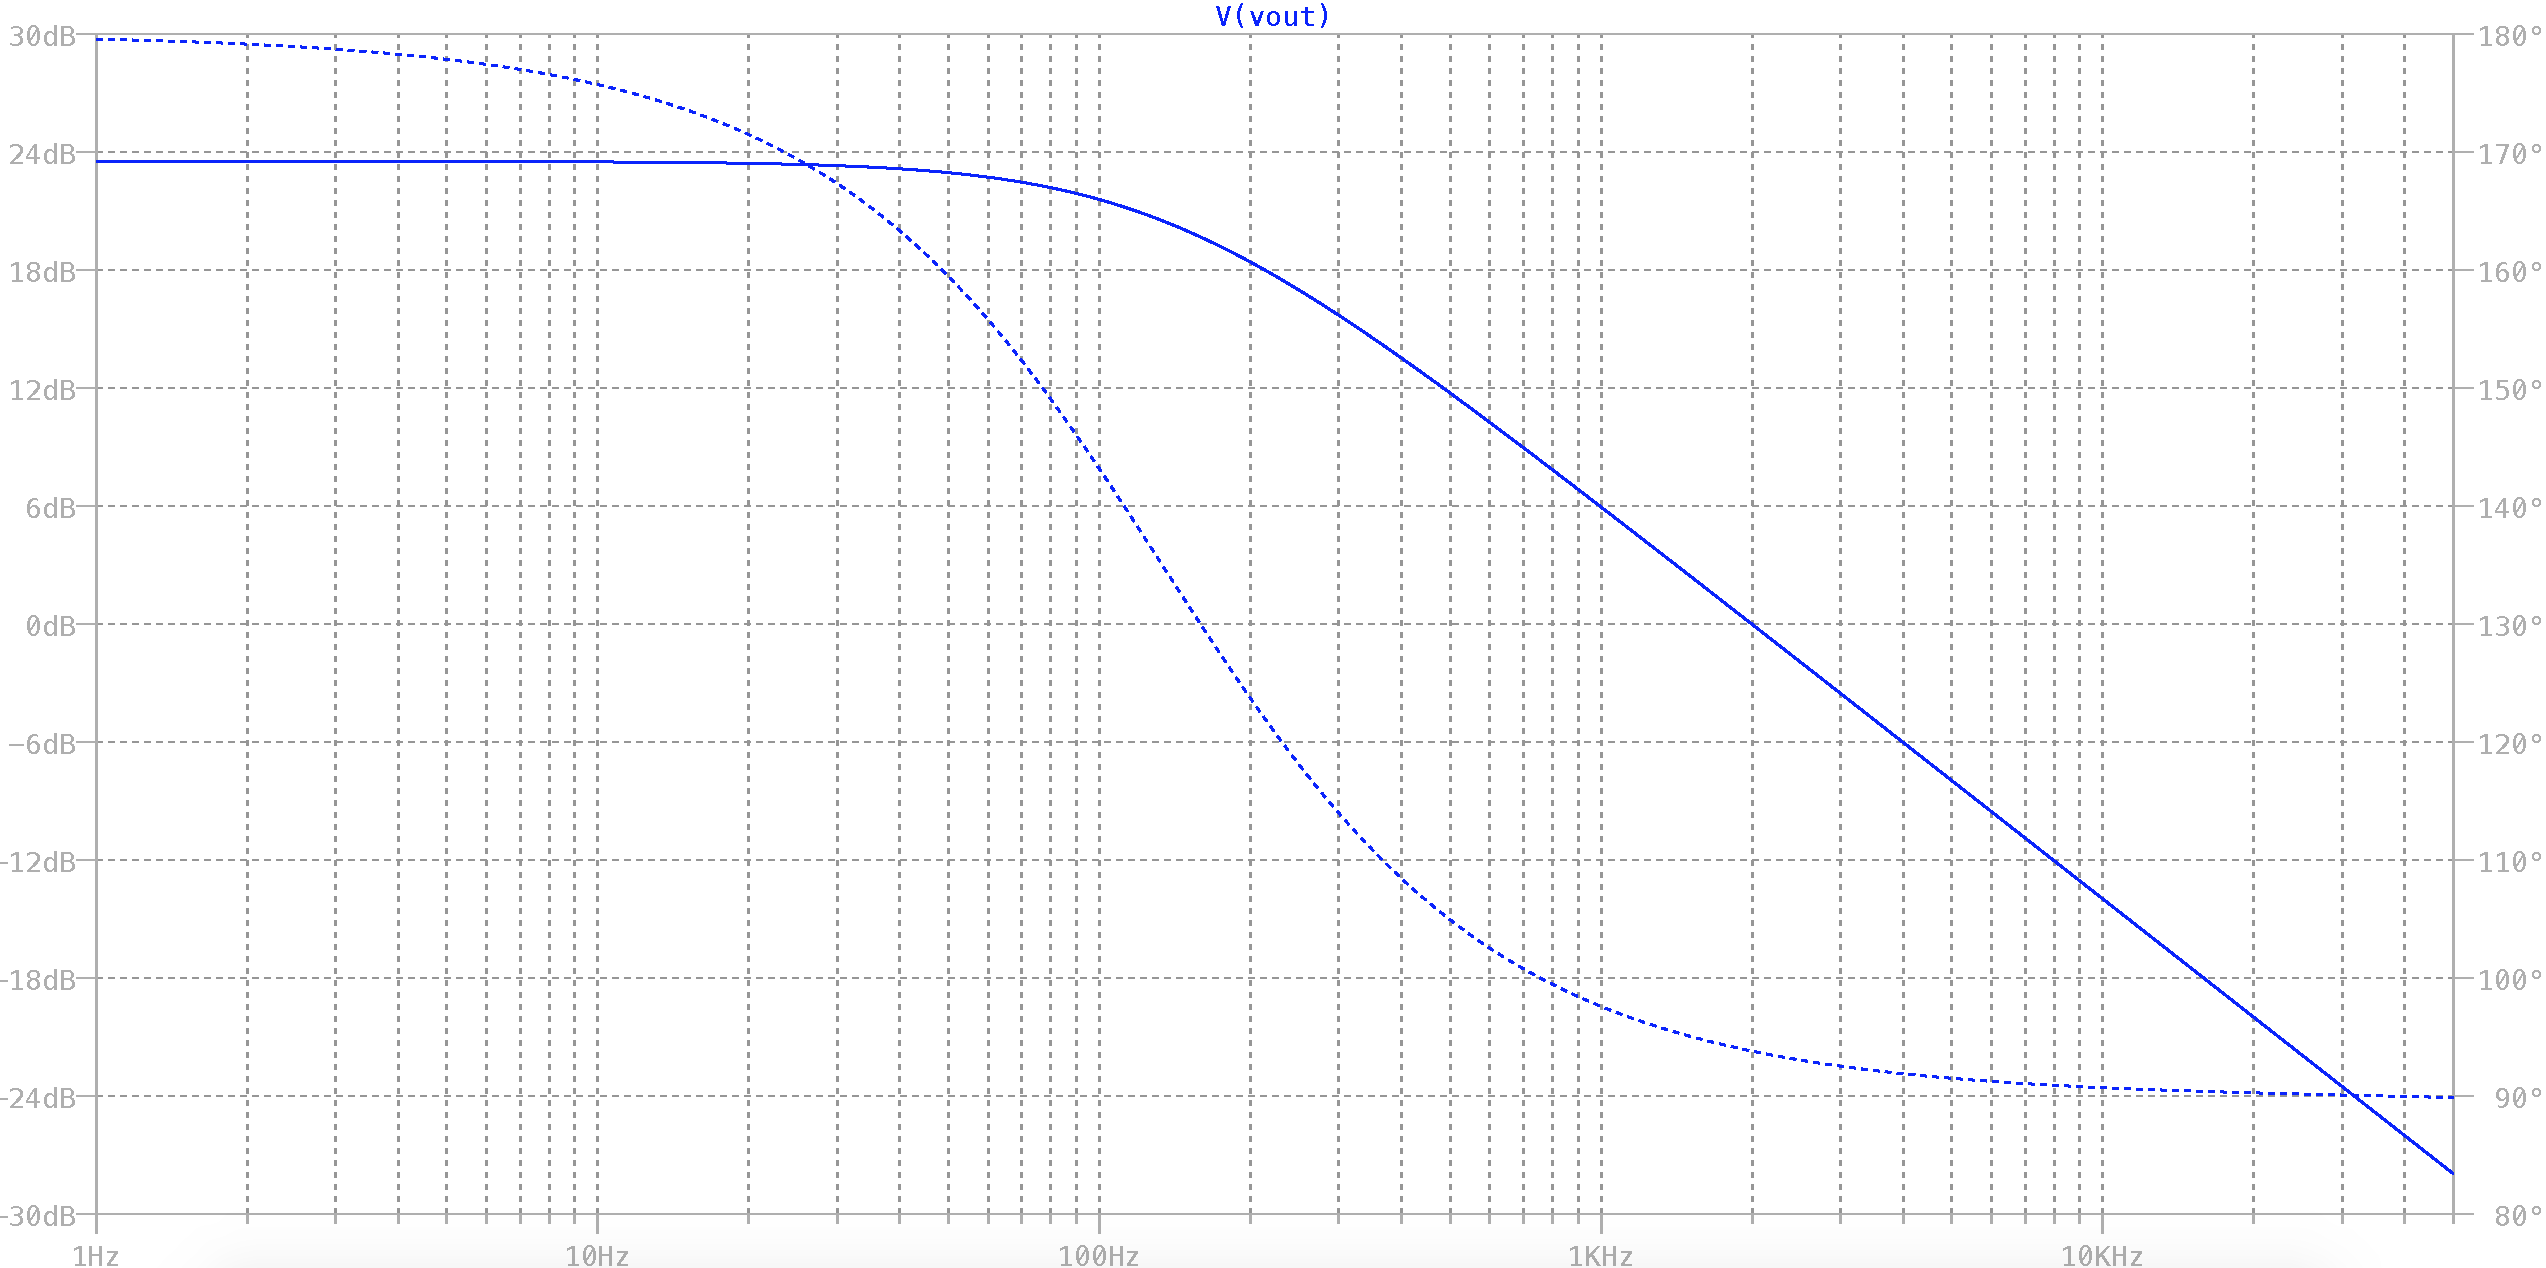
\includegraphics[scale=0.3]{sim_plot_fd}
      \caption{Phase and magnitude response of the practical integrator output}
    \end{figure}
    \begin{figure}[h]
      \centering
      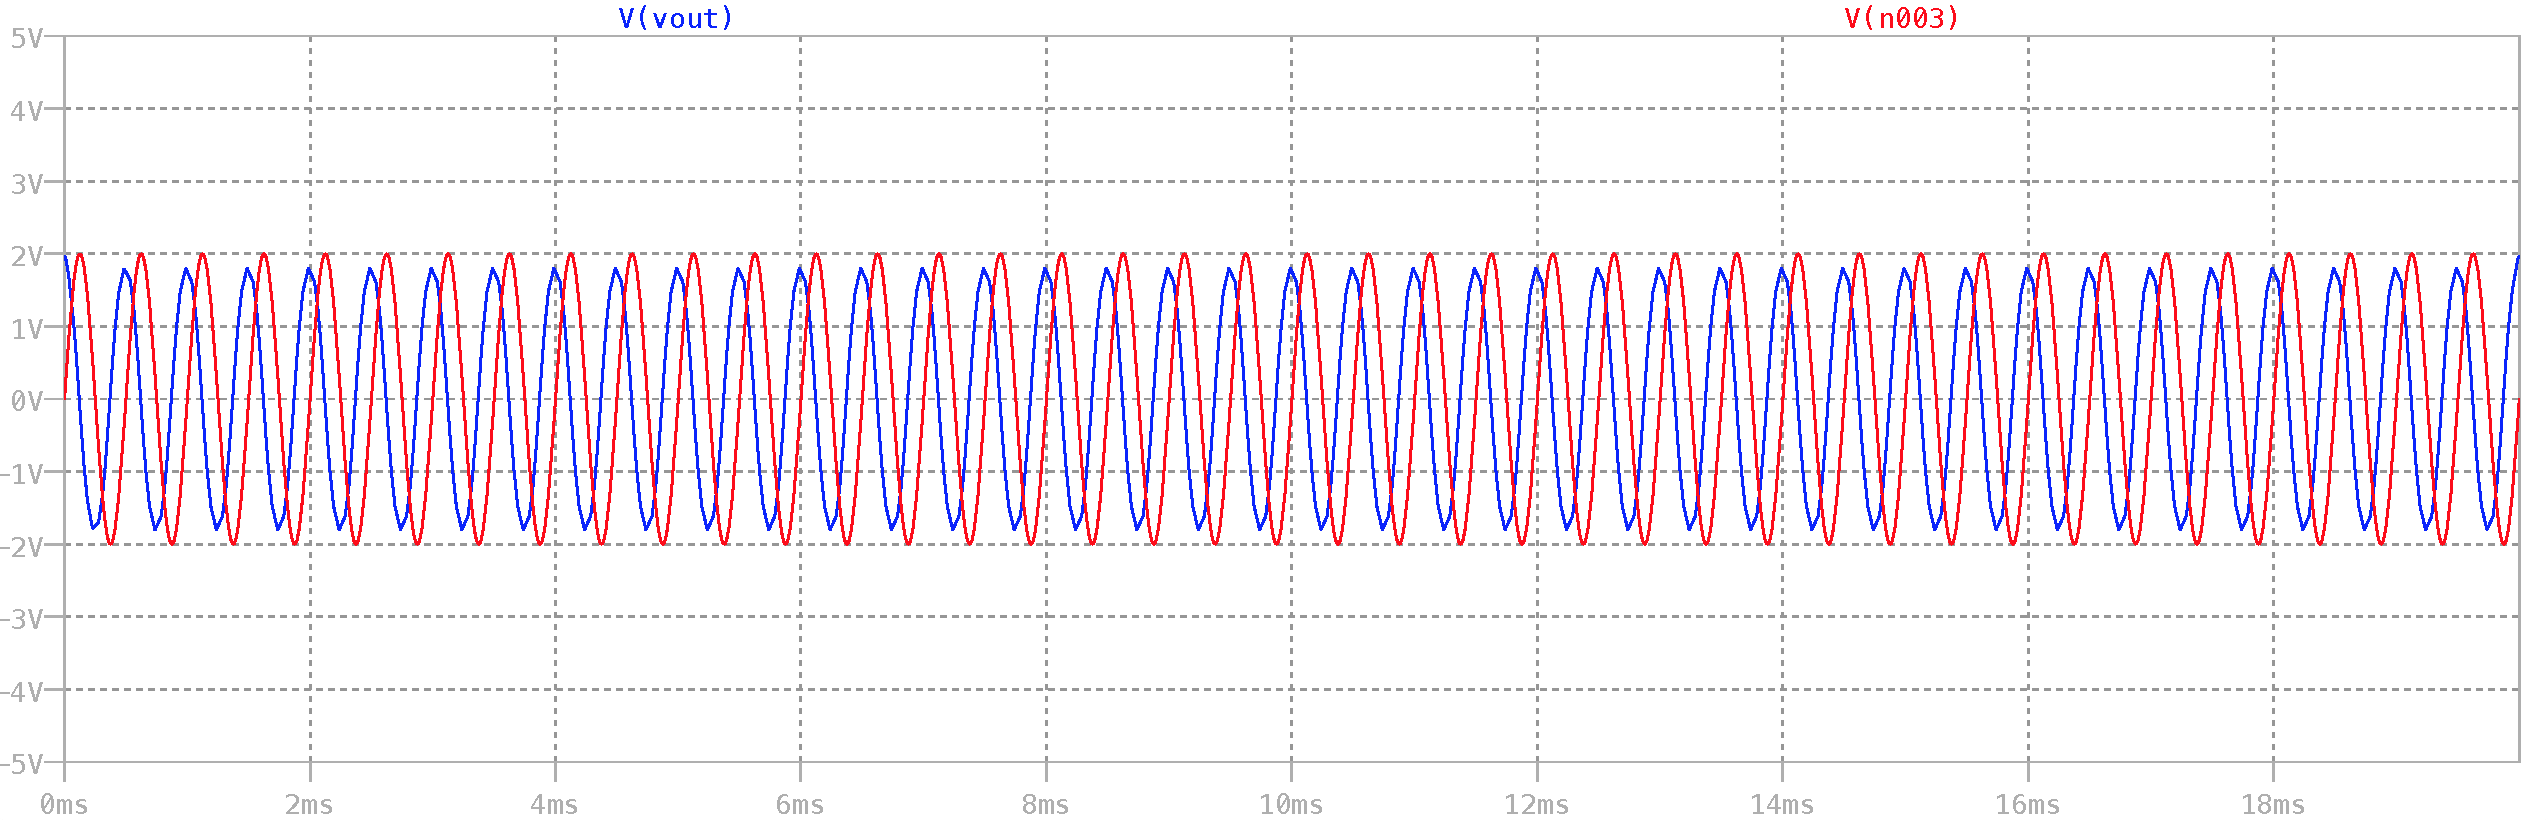
\includegraphics[scale=0.5]{sim_plot_td}
      \caption{\color{blue}$V_{out}$ \color{black}and \color{red}$V_{in}$ \color{black}in time domain}
    \end{figure}


  \newpage
  \section{Observations}
    %===A===
    \textbf{A}. The practical integrator is first designed based on the following constraints:
    Unity gain, $f_{-3dB} = f_{in}/15$ for a sinusoidal input
    $v_{in} = 2 sin(4000\pi t)$ and a phase error below 5\%.

    A leading phase sinusoidal wave appears at the output of the integrator as shown in figure \ref{fig:results_q1}.
    The DC gain, -3dB frequency $f_{3dB}$, unity gain frequency $f_u$, roll-off rate and phase shift are noted from the waveforms obtained on the DSO and the phase error is verified to be below 5\%.

    \begin{figure}[h]
      \centering
      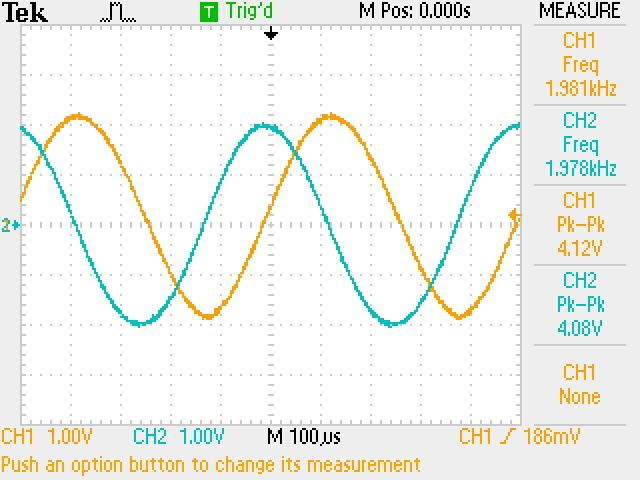
\includegraphics[scale=0.5]{images/results_q1.jpeg}
      \caption{Result \color{cyan}$V_{out}$ \color{black}of passing a sinusoidal input \color{orange}{$V_{in}$} \color{black}through the integrator.}
      \label{fig:results_q1}
    \end{figure}

    The observed parameters are listed below.
    \begin{itemize}
      \item[] DC gain = 14.89
      \item[] -3dB frequency $f_{-3dB}$ = 132 Hz
      \item[] Unity gain frequency $f_u$ = 2.07 kHz
      \item[] Roll-off rate = -18.35 dB/decade
      \item[] Phase shift $\phi$ = $1.608^{c}$ or $92.13^{\circ}$, an error of 2.4\%
    \end{itemize}

    \newpage
    %===B===
    \textbf{B}. The feedback resistor $R_F$ is then removed and the effect on the op-amp integrator configuration is observed.

    \begin{figure}[h]
      \centering
      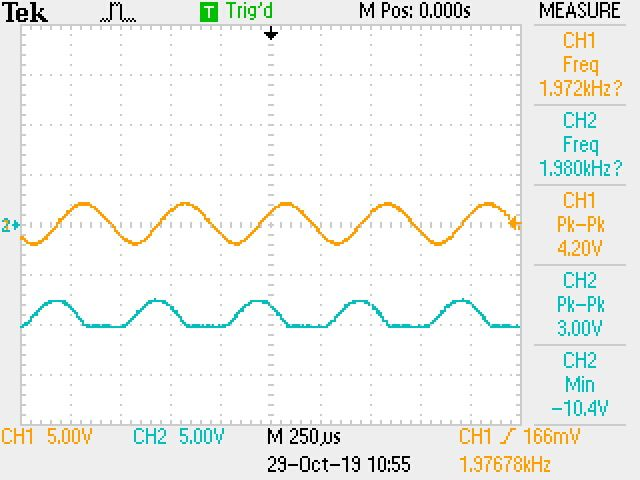
\includegraphics[scale=0.5]{images/results_q2.jpeg}
      \caption{The output \color{cyan}$V_{out}$ \color{black}saturates at low frequencies when $R_F$ is removed}
      \label{fig:results_q2}
    \end{figure}

    The output is given by $V_{out}=\pm V_{sat}$ as the capacitor acts as an open circuit at low frequencies as shown in figure \ref{fig:results_q2}. This sends the op-amp into an open loop configuraton.

    %===C===
    \textbf{C}. The sinusoidal input is replaced by a square wave of 4$V_{pk-pk}$ amplitude and a frequency of 2kHz to observe the integration operation of the configuration more clearly.

    A triangular waveform is obtained as a result of the square wave being integrated, as shown in figure \ref{fig:results_q3}.

    The peak-to-peak amplitude of the output can be obtained by using the relation
    $$ C\Delta V = I\Delta t$$
    Substituting $C=0.01\mu F$, $I=\cfrac{2}{8\times 10^3}$, $\Delta t = \cfrac{0.5}{2000}$,
    $$ \Delta V = 6.25 V$$
    Thus, the triangular waveform at the output is supposed to have a peak-to-peak voltage of $6.25$V and $6.32$V is observed as shown in figure \ref{fig:results_q3}.

    \textbf{D}. The frequency of the input is lowered to 130Hz and the output is observed again.

    \begin{figure}[!h]
      \centering
      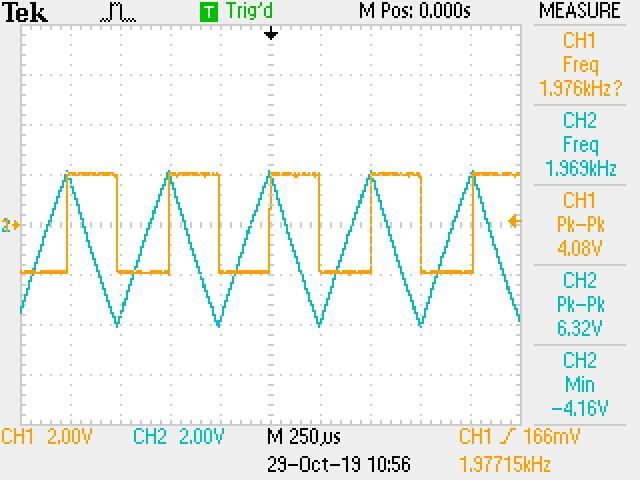
\includegraphics[scale=0.5]{images/results_q3.jpeg}
      \caption{Result \color{cyan}$V_{out}$ \color{black}of integrating a square wave \color{orange}$V_{in}$}
      \label{fig:results_q3}
    \end{figure}

    Using $ C\Delta V = I\Delta t$ and substituting $C=0.01\mu F$, $I=\cfrac{2}{8\times 10^3}$, $\Delta t = \cfrac{0.5}{130}$, we get:
    $$ \Delta V = 96.15 V$$
    Since $\Delta V > 2V_{sat}$ \text{, } $V_{out}$ gets clipped as shown in figure \ref{fig:results_q4}.

    \begin{figure}[!h]
      \centering
      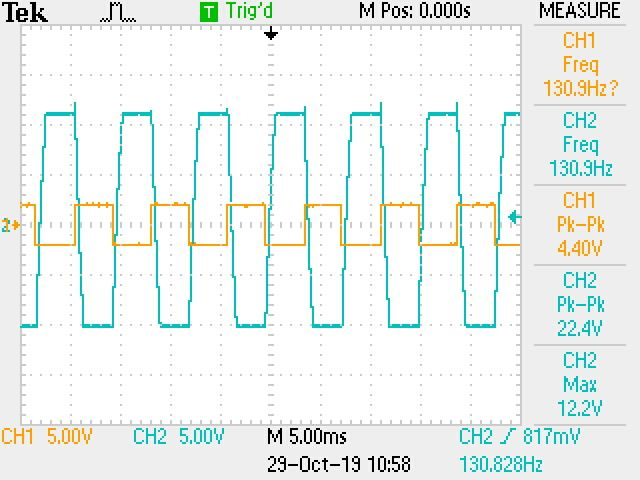
\includegraphics[scale=0.5]{images/results_q4_2.jpeg}
      \caption{Effect of lowering the input frequency on the output \color{cyan}$V_{out}$}
      \label{fig:results_q4}
    \end{figure}

  \clearpage
  \section{Results \& Conclusions}
  The op-amp based practical voltage integrator was designed subject to the given contraints, simulated in LTSpice and then implemented using the $\mu $A741 IC on a breadboard. The outputs were tested for sinusoidal and square wave at high and low input frequencies to understand the limitations of such a design.

  All the observations made during the testing of the physical circuit are listed below in brief.
  \begin{enumerate}
  \item The output waveform for the given sinusoidal input was obtained with a phase of $92.13^{\circ}$ resulting in a phase error of 2.4\%, well within the limit of 5\% specified in the given constraints.
  \item The ouput voltage was observed to saturate at $V_{sat}$ at low frequencies, when the resistor $R_{F}$ was removed.
  \item A triangular waveform was obtained when a square wave was given as input. This waveform was observed to be clipped at low frequencies.
  \end{enumerate}

  It can therefore be seen that an op-amp based practical integrator, which has a resistor $R_{F}$ in parallel with the capacitor $C$, overcomes the drawbacks of an ideal op-amp based integrator.

\end{document}
